\documentclass[anonymous, a4paper, UKenglish, cleveref, autoref, thm-restate]{lipics-v2021}
\usepackage[utf8]{inputenc} % Required for inputting international characters
\usepackage[T1]{fontenc} % Output font encoding for international characters
% \usepackage[backend=bibtex,style=alphabetic,natbib=true]{biblatex}
% \usepackage[backend=bibtex,style=alphabetic,natbib=true]{biblatex}
% \addbibresource{references.bib}
\usepackage{amsmath, amssymb, amsfonts, amsthm, stmaryrd}
\usepackage{caption}
\usepackage{subcaption}
\usepackage{graphicx}
\usepackage{enumitem}
\usepackage{mathpartir}
\usepackage{bussproofs}
\usepackage{xparse}
\usepackage[usenames, dvipsnames]{xcolor}
\usepackage{lipsum}
\usepackage{xargs}
\usepackage{hyperref}
\usepackage{tikz-cd}
\usepackage{todonotes}
\usepackage{url}
\usepackage{xspace}
\usepackage{rotating}
\usepackage{quiver}
\usepackage{minted}
\usepackage{newunicodechar}
\usepackage{microtype}
% \addbibresource{references.bib}
\usepackage{array}   % for \newcolumntype macro
\newcolumntype{C}{>{$}c<{$}} % math-mode version of "l" column type
\newcolumntype{L}{>{$}l<{$}} % math-mode version of "l" column type

% \usepackage{draftwatermark}
% \SetWatermarkText{Confidential}
% \SetWatermarkScale{4}
% \SetWatermarkColor[gray]{0.9}

\hypersetup{
  linktocpage,
  colorlinks,
  citecolor=BlueViolet,
  filecolor=red,
  linkcolor=Blue,
  urlcolor=BrickRed
}
\newcommand{\mpav}[1]{\textcolor{red}{\textsc{Marco}: #1}}
\newcommand{\dcas}[1]{\textcolor{ForestGreen}{\textsc{David}: #1}}
\newcommand{\mvol}[1]{\textcolor{blue}{\textsc{Michael}: #1}}
\newcommand{\proofcomment}[1]{\text{\{ #1 \}}}
\newenvironment{proofof}[1] {\begin{proof}[Proof of {#1}]}{\end{proof}}
\newcommand{\eqdef}{\stackrel{\mathrm{\Delta}}{=}}
\newcommand{\bnfeq}{\mathrel{::=}}
\newcommand{\defeq}{\triangleq}
\newcommand{\rul}[3]{\frac{#2}{#3}\;  {\textrulelabel{#1}}}
\newcommand{\den}[1]{\llbracket #1 \rrbracket}
\newcommand{\jud}[3]{#1 \vdash #2 : #3}
\newcommand{\bden}[1]{\llparenthesis#1 \rrparenthesis}
\newcommand{\bigslant}[2]{{\raisebox{.2em}{$#1$}\left/\raisebox{-.2em}{$#2$}\right.}}
\newcommand{\quotient}[2]{\bigslant{#1}{#2}}
\newcommand{\curry}{\Lambda}
\newcommand{\uncurry}{\begin{sideways}\begin{sideways}$\Lambda$\end{sideways}\end{sideways}}
\newcommand{\Bool}{\mathbb{B}}
\newcommand{\N}{\mathbb{N}}
\newcommand{\Nat}{\N}
\newcommand{\R}{\mathbb{R}}
\newcommand{\Sets}{\mathbf{Set}}
\newcommand{\blacklater}{\blacktriangleright}
\newcommand{\tot}{\mathcal{S}}
\newcommand{\PSh}{\ensuremath{\textbf{PSh}(\omega)}}

\newsavebox{\lbananabox}
\newcommand{\lbananamacro}{%
  
\begin{tikzpicture}[baseline=0.25em,xscale=0.005em,yscale=0.005em]
  \draw[solid, join=round] (2,0) to[out=140,in=-90] (0,3) to[out=90,in=-140] (2,6) -- (2.1,5.9)
              to[out=-120,in=90] (1.2,3) to[out=-90,in=120] (2.1,0.1) -- cycle;
\end{tikzpicture}
}
\savebox{\lbananabox}{\lbananamacro}
\newcommand{\lbanana}{\mathopen{\usebox{\lbananabox}\hspace{-0.6ex}}}


\newsavebox{\rbananabox}
\newcommand{\rbananamacro}{%
  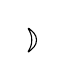
\begin{tikzpicture}[baseline=0.25em,xscale=-0.005em,yscale=0.005em]
  \draw[solid, join=round] (2,0) to[out=140,in=-90] (0,3) to[out=90,in=-140] (2,6) -- (2.1,5.9)
              to[out=-120,in=90] (1.2,3) to[out=-90,in=120] (2.1,0.1) -- cycle;
  \end{tikzpicture}
}
\savebox{\rbananabox}{\rbananamacro}
\newcommand{\rbanana}{\mathclose{\usebox{\rbananabox}}}


\newsavebox{\lbansbox}
\newcommand{\lbansmacro}{%
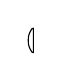
\begin{tikzpicture}[baseline=0.45ex,xscale=0.006em,yscale=0.012ex]%
% curvey bananas
%\draw[solid,join=round,fill=yellow] (2,0) to[out=140,in=-90] (0,3) to[out=90,in=-140] (2,6) -- (2.1,5.9) to[out=-120,in=90] (1.2,3) to[out=-90,in=120] (2.1,0.1) -- cycle;%
% fitted lenses
\draw[solid,join=round] (1.8,6) -- (1.5,5.9) to[out=-120, in=90] (0.7,3) to[out=-90, in=120] (1.5,0.1) -- (1.8,0) -- cycle;%
\end{tikzpicture}}
\savebox{\lbansbox}{\lbansmacro}
\newcommand{\lbans}{\mathopen{\usebox{\lbansbox}\mspace{1mu}}}

\newsavebox{\rbansbox}
\newcommand{\rbansmacro}{%
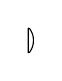
\begin{tikzpicture}[baseline=0.45ex,xscale=-0.006em,yscale=0.012ex]%
% curvey bananas
%\draw[solid,join=round,fill=yellow] (2,0) to[out=140,in=-90] (0,3) to[out=90,in=-140] (2,6) -- (2.1,5.9) to[out=-120,in=90] (1.2,3) to[out=-90,in=120] (2.1,0.1) -- cycle;%
% fitted lenses
\draw[solid,join=round] (1.8,6) -- (1.5,5.9) to[out=-120, in=90] (0.7,3) to[out=-90, in=120] (1.5,0.1) -- (1.8,0) -- cycle;%
\end{tikzpicture}}
\savebox{\rbansbox}{\rbansmacro}
\newcommand{\rbans}{\mathclose{\mspace{1mu}\usebox{\rbansbox}}}

\newsavebox{\llensbox}
\newcommand{\llensmacro}{%
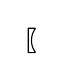
\begin{tikzpicture}[baseline=0.45ex,xscale=0.006em,yscale=0.012ex]%
\draw[solid,join=round] (1.4,0) -- (0,0) -- (0,6) -- (1.4,6) -- (1.5,5.9) to[out=-120, in=90] (0.7,3) to[out=-90, in=120] (1.5,0.1) -- cycle;%
\end{tikzpicture}}
\savebox{\llensbox}{\llensmacro}
\newcommand{\llens}{\mathopen{\usebox{\llensbox}\mspace{1mu}}}

\newsavebox{\rlensbox}
\newcommand{\rlensmacro}{%
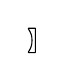
\begin{tikzpicture}[baseline=0.45ex,xscale=-0.006em,yscale=0.012ex]%
\draw[solid,join=round] (1.4,0) -- (0,0) -- (0,6) -- (1.4,6) -- (1.5,5.9) to[out=-120, in=90] (0.7,3) to[out=-90, in=120] (1.5,0.1) -- cycle;%
\end{tikzpicture}}
\savebox{\rlensbox}{\rlensmacro}
\newcommand{\rlens}{\mathclose{\mspace{1mu}\usebox{\rlensbox}}}

% filled versions
\newcommand{\Lbanana}{%
  \mathopen{\mspace{1mu}\tikz[baseline=0.25em,xscale=0.006em,yscale=0.006em]
  \fill (2,0) to[out=140,in=-90] (0,3) to[out=90,in=-140] (2,6) -- (2.1,5.9)
              to[out=-120,in=90] (1.2,3) to[out=-90,in=120] (2.1,0.1) -- cycle;\mspace{1mu}}}
\newcommand{\Rbanana}{%
  \mathclose{\mspace{1mu}\tikz[baseline=0.25em,xscale=-0.006em,yscale=0.006em]
  \fill (2,0) to[out=140,in=-90] (0,3) to[out=90,in=-140] (2,6) -- (2.1,5.9)
              to[out=-120,in=90] (1.2,3) to[out=-90,in=120] (2.1,0.1) -- cycle;}}
% % lens brackets (using TikZ)
% \newcommand{\llens}{%
%   \mathopen{\tikz[baseline=0.25em,xscale=0.006em,yscale=0.006em]
%   \draw[join=round] (1.4,0) -- (0,0) -- (0,6) -- (1.4,6) -- (1.5,5.9)
%         to[out=-120,in=90] (0.7,3) to[out=-90,in=120] (1.5,0.1) -- cycle;\mspace{1mu}}}
% \newcommand{\rlens}{%
%   \mathclose{\mspace{1mu}\tikz[baseline=0.25em,xscale=-0.006em,yscale=0.006em]
%   \draw[join=round] (1.4,0) -- (0,0) -- (0,6) -- (1.4,6) -- (1.5,5.9)
%         to[out=-120,in=90] (0.7,3) to[out=-90,in=120] (1.5,0.1) -- cycle;}}
% filled versions
\newcommand{\Llens}{%
  \mathopen{\tikz[baseline=0.25em,xscale=0.006em,yscale=0.006em]
  \fill (1.4,0) -- (0,0) -- (0,6) -- (1.4,6) -- (1.5,5.9)
        to[out=-120,in=90] (0.7,3) to[out=-90,in=120] (1.5,0.1) -- cycle;\mspace{1mu}}}
\newcommand{\Rlens}{%
  \mathclose{\mspace{1mu}\tikz[baseline=0.25em,xscale=-0.006em,yscale=0.006em]
  \fill (1.4,0) -- (0,0) -- (0,6) -- (1.4,6) -- (1.5,5.9)
        to[out=-120,in=90] (0.7,3) to[out=-90,in=120] (1.5,0.1) -- cycle;}}


\newcommand{\anamor}[1]{{\llens\, #1\, \rlens}}
\newcommand{\catamor}[1]{\lbans\, #1\, \rbans}
\newcommand{\cata}[1]{\lbans #1 \rbans}
\newcommand{\ana}[1]{\llens #1 \rlens}
\newcommand{\catafree}[1]{\Lbanana #1 \Rbanana}
\newcommand{\anacofree}[1]{\Llens #1 \Rlens}
\newcommand{\hylo}[2]{\cata{#1 \to #2}}
\newcommand{\cohylo}[2]{\ana{#1 \to #2}}
\newcommand{\fold}[1]{\catamor{#1}}
\newcommand{\unfold}[1]{\anamor{#1}}
\newcommand{\comp}{\cdot}
\newcommand{\operator}[1]{\textsf{#1}}
\newcommand{\head}{\operator{head}}
\newcommand{\inl}{\operator{inl}}
\newcommand{\inr}{\operator{inr}}
\newcommand{\tail}{\operator{tail}}
\newcommand{\Alg}{\text{-Alg}}
\newcommand{\Free}{\text{Free\xspace}}
\newcommand{\fmap}[1]{\text{fmap}\;#1}

\newcommand{\zero}{\operator{zero}}
\newcommand{\Nil}{\operator{nil}}
\newcommand{\Succ}{\operator{succ}}

\newcommand{\InOp}{\operator{in}^{\circ}}
\newcommand{\InIso}{\operator{in}}
\newcommand{\OutOp}{\operator{out}^{\circ}}
\newcommand{\OutIso}{\operator{out}}
\newcommand{\call}{\operator{call}}

\newcommand{\CatC}{\mathcal{C}}
\newcommand{\CatD}{\mathcal{D}}
\newcommand{\CatE}{\mathcal{E}}
\newcommand{\CatI}{\mathcal{I}}
\newcommand{\Set}{\mathbf{Set}}
\newcommand{\iso}{\cong}
\newcommand{\ceiling}[1]{\lceil #1 \rceil}
\newcommand{\floor}[1]{\lfloor #1 \rfloor}
\newcommand{\pair}[2]{\langle #1, #2 \rangle}
\newcommand{\haskell}[1]{\mintinline{haskell}{#1}}

%\newcommand{\coq}[1]{\mintinline{coq}{#1}}
\newmintinline[coq]{coq}{fontsize=\small}
\newminted{coq}{fontsize=\small}

\title{A Mechanised Library for Generic (Co)Programming}

\bibliographystyle{plainurl}% the mandatory bibstyle
%\titlerunning{Dummy short title} %TODO optional, please use if title is longer than one line

\author{David Castro-Perez}{School of Computing, University of Kent}{d-castro-perez@kent.ac.uk}{}{}
\author{Marco Paviotti}{School of Computing, University of Kent}{m.paviotti@kent.ac.uk}{}{}
\author{Michael Vollmer}{School of Computing, University of Kent}{m.vollmer@kent.ac.uk}{}{}

%\author{Jane {Open Access}}{Dummy University Computing Laboratory, [optional: Address], Country \and My second affiliation, Country \and \url{http://www.myhomepage.edu} }{johnqpublic@dummyuni.org}{https://orcid.org/0000-0002-1825-0097}{(Optional) author-specific funding acknowledgements}%TODO mandatory, please use full name; only 1 author per \author macro; first two parameters are mandatory, other parameters can be empty. Please provide at least the name of the affiliation and the country. The full address is optional. Use additional curly braces to indicate the correct name splitting when the last name consists of multiple name parts.

%\author{Joan R. Public\footnote{Optional footnote, e.g. to mark corresponding author}}{Department of Informatics, Dummy College, [optional: Address], Country}{joanrpublic@dummycollege.org}{[orcid]}{[funding]}

\authorrunning{D. Castro-Perez, M. Paviotti, and M. Vollmer} %TODO mandatory. First: Use abbreviated first/middle names. Second (only in severe cases): Use first author plus 'et al.'

\Copyright{D. Castro-Perez, M. Paviotti, and M. Vollmer} %TODO mandatory, please use full first names. LIPIcs license is "CC-BY";  http://creativecommons.org/licenses/by/3.0/

\ccsdesc[100]{\textcolor{red}{Replace ccsdesc macro with valid one}} %TODO mandatory: Please choose ACM 2012 classifications from https://dl.acm.org/ccs/ccs_flat.cfm 

\keywords{hylomorphisms, Coq, code extraction, verification} %TODO mandatory; please add comma-separated list of keywords

\category{} %optional, e.g. invited paper

\relatedversion{} %optional, e.g. full version hosted on arXiv, HAL, or other respository/website
%\relatedversiondetails[linktext={opt. text shown instead of the URL}, cite=DBLP:books/mk/GrayR93]{Classification (e.g. Full Version, Extended Version, Previous Version}{URL to related version} %linktext and cite are optional

%\supplement{}%optional, e.g. related research data, source code, ... hosted on a repository like zenodo, figshare, GitHub, ...
%\supplementdetails[linktext={opt. text shown instead of the URL}, cite=DBLP:books/mk/GrayR93, subcategory={Description, Subcategory}, swhid={Software Heritage Identifier}]{General Classification (e.g. Software, Dataset, Model, ...)}{URL to related version} %linktext, cite, and subcategory are optional

%\funding{(Optional) general funding statement \dots}%optional, to capture a funding statement, which applies to all authors. Please enter author specific funding statements as fifth argument of the \author macro.

%\acknowledgements{I want to thank \dots}%optional

%\nolinenumbers %uncomment to disable line numbering



%Editor-only macros:: begin (do not touch as author)%%%%%%%%%%%%%%%%%%%%%%%%%%%%%%%%%%
\EventEditors{John Q. Open and Joan R. Access}
\EventNoEds{2}
\EventLongTitle{42nd Conference on Very Important Topics (CVIT 2016)}
\EventShortTitle{CVIT 2016}
\EventAcronym{CVIT}
\EventYear{2016}
\EventDate{December 24--27, 2016}
\EventLocation{Little Whinging, United Kingdom}
\EventLogo{}
\SeriesVolume{42}
\ArticleNo{23}
%%%%%%%%%%%%%%%%%%%%%%%%%%%%%%%%%%%%%%%%%%%%%%%%%%%%%%

\begin{document}

\maketitle

%TODO mandatory: add short abstract of the document
\begin{abstract}

\end{abstract}

\section{Introduction}
\label{sec:intro}
Recursive definitions cannot be proven well-defined automatically due to the
halting problem. Modern proof assistants like Coq or Agda provide a sound, but
incomplete algorithm which syntactically checks for termination or productivity.
For recursion, this is done by trying to (automatically) infer which argument in
the recursive call gets smaller with respects to the original input argument.
For productivity, the algorithm checks that the (co)recursive call appears
directly under a constructor to make sure that this function always produce at
least one element after each recursive step.

As mentioned, some functions, though well-defined, cannot be accepted by the
proof assistant. One example is the quicksort algorithm. This is given by the
\haskell{partition} and \haskell{quicksort} function below (written in Haskell
code):
While \haskell{quicksort} is a well-defined mathematical function it cannot be
accepted by a proof assistant.  The reason is that the \haskell{partition}
function \emph{destructuring} the input ``dives'' deeper in the input returning
two sublists with the head as a pivot.

A pen-and-paper technique would be to show that the \haskell{partition} is a
\emph{well-founded coalgebra} on the functor $(- \times A \times -)$ for a fixed
type $A$. Here the term ``well-founded'' refers to the fact that the infinite
iteration of this coalgebra will produce a \emph{finite} binary tree with nodes
in $A$.

More generally, this is an instance of a \emph{divide-and-conquer} algorithm.
Such algorithms are structured in three parts: first, the input is broken down
in smaller sub-problems by means of a well-founded coalgebra. Secondly, these
sub-problems are computed recursively and, finally, the results of the recursive
call are put together by a an algebra. This particular way of doing recursion
has been named in the functional programming literature as a
hylomorphism~\cite{MeijerFP91, HuIT96}.

Many years later Hinze et al.~\cite{HinzeWG15} showed that every recursive
program can be turned into an hylomorphism by means of the conjugate rule. The
essence of this result is that every complex recursion scheme can be explained
by its associated \emph{adjunction} which establishes a way of reducing the
proof obligation for the complex recursion scheme into the proof obligation for
a basic hylomorphism. This can be paraphrased by saying
\begin{center}
  ``\emph{every recursion scheme can be formalised as an hylomorphism}''
\end{center}

This result has given a much needed unifying view of recursion scheme which
helped understanding their nature and also in providing a unified way of
reasoning about recursive programs by means of fusion laws.

\dcas{My take would be different here from now on. See below:}

Recursion schemes enjoy generic algebraic laws for program manipulation. Many
common optimisations and transformations are instances of such laws. Examples of
this include shortcut deforestation~\cite{TakanoM95}, and
parallelisations~\cite{Gibbons96:Third}. \dcas{TODO: add more examples?}

With this work, we study the formalisation of hylomorphism laws in proof
assistants like Coq to derive efficient and correct recursive algorithms by
program calculation techniques. Furthermore, our encoding of hylomorphisms
allows Coq's code extraction mechanism to produce OCaml code that resembles what
a programmer would have writen manually.

\dcas{END (TODO: merge with Marco's. I would omit (or take parts of the) below)}

There is a tension:
\begin{itemize}
  \item On one hand we can allow general recursion and the employ recursion
schemes to help the programmer structuring programs so that they terminate
  \item on the other hand we could forbid non-termination, but at this point
there is no algorithm to tell termination and non-termination apart.
\end{itemize}

The type theoretical approach instead is to reject all definitions which cannot
be proven well-defined. It is safer, but incomplete.

With this work we intend to begin a study of the applications of recursion
schemes that goes beyond functional programming, that is to dependent type
theories such as a the ones employed in proof assistants like Agda or Coq where
non-termination is outright rejected.

This has been a long-standing challenge to come up with a sound algorithm which
rejects all programs that do not terminate (soundness) and accepts as many
well-defined programs as possible (completeness). Our aim is to provide an
additional tool to the every-day programmer to be able to extend the range of
recursive programs we can write.
\mvol{What is the ``every-day programmer'' here? Are they working in Coq/Agda?}

\dcas{Note: the below is useful to keep in the intro}
One of the challenges here is to be able to keep the theory of recursions
schemes as general as possible while maintaining its practical usefulness. In
order to do this, we have to make some design choices which differ a bit from
the general theory.  For instance, formalising the conjugate rule would require
us to mechanise a non-trivial fragment of category theory inside the prover's
logic.  Secondly, the general conjugate rule is a statement of correspondence of
arrows rather than a proof that these programs actually exists. In functional
programming languages like for instance Haskell this is not a problem, since
every functor is strong and has a fixed-point.  On the other hand, in a type
theory we have to restrict to those so-called polynomial functors. In this work
we do not make use of these assumptions. By restricting ourselves to polynomial
functors given in terms of containers~\cite{AbbottAG05} we are able to prove the
recursion schemes within the proof assistant and at the same time to maintain a
certain level of data abstraction.

First we prove that the hylo equation has a unique solution
\[
  x = a \comp F(x) \comp c
\]
for every recursive coalgebra $c$ for a polynomial $F$. Then we prove each
recursion scheme by reducing it to a hylo. The following recursion schemes can
all be proven by reducing them to an hylo: folds, mutual recursive functions,
recursion schemes from comonads and their respective coinductive dual.
\mpav{Moved this from Section 3}

\mvol{Need some transiiton here to build up to listing the goals and contributions of the paper. Also, ``axiom-free'' and ``obj.magic'' come out of nowhere here, so both need to be established earlier in the introduction.}
The primary goals of this work are:
\begin{enumerate}
  \item that the
  mechanisation of hylomorphisms and their laws should be axiom-free; and
  \item that Coq
hylomorphisms should be extracted to recursive OCaml functions that use no
instances of \mintinline{OCaml}{Obj.magic}.
\end{enumerate}
In OCaml, \mintinline{OCaml}{Obj.magic} allows for unsafe casts between types.
Although the use of \mintinline{OCaml}{Obj.magic} should be safe in the code
extracted by Coq, it has been proven that, for higher-order programs, simple
interoperations can lead to incorrect behaviour or even
segfaults~\cite{forster:hal-04329663}. Therefore, the avoidance of axioms and
\mintinline{OCaml}{Obj.magic} means that the extracted code will have stronger
safety guarantees, and will allow the safe interoperation with other OCaml code.
\mvol{This is good!}

The contributions we make in this paper are as follows:
\begin{itemize}
  \item We provide a framework for \emph{generic programming} with recursion
schemes in Coq
  \item We formalise algorithms for divide and conquer, dynamic programming and
mutual recursion
  \item We validated optimisations in Coq and extract the resulting code to
OCaml.
\end{itemize}

\section{Background on Recursion Schemes}
Recursion schemes provide a systematic way to work with data types, such as
trees or lists, by abstracting away the recursion into higher-order functions.
Canonical recursion schemes include \emph{folds} (catamorphisms) which consume
data and \emph{unfolds} (anamorphisms) which produce data. These are the unique
solutions (when they exist) to the following two equations respectively
\[
  h  = a \comp F h \comp \InOp \qquad k = \OutOp \comp F k \comp c
\]
where $F$ is a \emph{base functor}, $Ff$ is the \emph{functorial action} which
can be thought of the program $\operator{fmap}\; f$, $a$ is a program of type
$F A \to A$ (an $F$-algebra),  $c$ is a program of type $C \to FC$ (a
$F$-coalgebra), $\InOp$ is the isomoprhism on the least fixed-point of $F$,
namely $\InOp : \mu F \to F\mu F$, and $\OutOp$ is the isomorphism on
the greatest fixed-point of $F$, namely $F \nu F \to \nu F$. When
the unique solutions to the above equations exist we denote them as $\cata{a}$
and $\ana{c}$ respectively.

\subsection{Hylomorphisms}
Catamorphisms (dually anamorphisms) do not capture every recursion
scheme we can think of.  As an example, consider an example of a classic
\emph{divide-and-conquer} program such as quicksort algorithm:\footnote[1]{This
program is written in Coq notation to be consistent, but it is not a program
that Coq can accept.}

\mpav{I need this to be written in Coq notation}
\begin{coqcode}
qs :: [a] -> [a]
qs [] = []
qs (x:xs) = qs (filter (x <=) xs) ++ [x] ++ (qs (filter (x >) xs))
\end{coqcode}
This program is formed of essentially two parts. The first one is what is
commonly thought as the \emph{partition} function destructuring the input list
in three parts, the pivot and the other two sublists, and the second part
recursing over the sublists and composing the results back together.

Notice that if we define the functor \coq{TreeF} $X = X \times A \times X$ with
the obvious functorial action then \coq{partition} can be viewed as a
\coq{TreeF}-coalgebra on lists over the type $A$
\begin{coqcode}
c : [A] -> TreeF [A]
c (x:xs) = (filter (x <=) xs, x, filter (x >) xs)
\end{coqcode}

While we can define an \coq{TreeF}-algebra on lists
over $A$ as well, that is a map
\begin{coqcode}
a : TreeF [A] -> [A]
a (left, x, right) = left ++ [x] ++ right
\end{coqcode}

It should be easy to see that the program \coq{qs} can now be defined as the
unique program that runs the coalgebra $c$ recurses over the sublists produced
and then composes the results together. The structure exemplified by this
program is a typical divide-and-conquer algorithm which can be implemented using
an \emph{hylomorphism}. An hylomorphism is the unique solution $x : C \to A$ to
the hylo equation
\begin{equation}
  \label{eq:hylo}
  x =  a \comp Fx \comp c
\end{equation}
for a $F$-algebra on $A$, an $F$-coalgebra on $C$ and a functor $F$.  If for
every $F$-algebra there exists a unique solution to (\ref{eq:hylo}) then we say
the $F$-coalgebra $c$ is \emph{recursive}. Dually if for every $F$-coalgebra $c$
there exists a unique solution to (\ref{eq:hylo}) we say the $F$-algebra $a$ is
\emph{corecursive}. We denote the unique solution to the hylo equation
(\ref{eq:hylo}) as $\hylo{a}{c}$.

Moreover, it shoud be easy to see that catamorphisms and anamorphism arise as a
special case of hylomorphisms
\begin{equation}
  \label{eq:cata}
  \cata{a} = \hylo{\InOp}{a} \qquad \ana{c} = \hylo{c}{\OutOp}
\end{equation}
since $\InOp$ is indeed a recursive coalgebra and $\OutOp$ is a corecursive
algebra.

\subsection{Implementing Recursion Schemes}
Hylomorphisms can implement all structured recursion schemes~\cite{HinzeWG15,
HinzeW16}.  Here we show the result by means of a very basic example: mutual
recursion. We refer the reader to Hinze et al.~\cite{HinzeWG15} for the
theoretical result and to Yang and Wu~\cite{YangW22} for more examples of
recursion schemes.

% More specifically, in the context of recursive data types, such as in Haskell,
% where induction and coinduction is conflated, an hylomorphism can be implemented
% in terms of a catarmorphism (folding) and an anamorphism (unfolding)
% \[
%   \hylo{a}{c} = \cata{a} \comp \ana{c}
% \]
% They first generate a data structure using an anamorphism and then immediately
% fold or reduce it using a catamorphism.

% The hylomorphism pattern is particularly useful for defining recursive
% algorithms in a functional programming context, where recursion is a fundamental
% tool for solving problems. By separating the generation of data structures from
% their consumption, hylomorphisms enable clearer and more modular code, making it
% easier to reason about and maintain recursive algorithms.

% However, in a type theory inductive and coinductive data types are separate.

% In this section we will introduce the notion of hylomorphism. By way of examples
% we will also give high level intution as to way all recursion schemes can be
% defined in terms of a basic

Say that we want to prove that the two mutually recursive functions below are
well-defined

\begin{tabular}{LL}
  \operator{even} : \Nat \to \Bool                  &  \operator{odd} : \Nat \to \Bool\\
  \operator{even} (0) = \top                        &  \operator{odd}(0) = \bot\\
  \operator{even} (n+1) = \neg \operator{odd}(n)    &  \operator{odd}(n+1) = \neg (\operator{even}(n))
\end{tabular}

One option is to prove that the following function is
equivalent to the above
\begin{align*}
  & \operator{even-odd} : \Nat \to \Bool \times \Bool\\
  & \operator{even-odd} (0) = (\top, \bot)\\
  & \operator{even-odd} (n+1) = \operator{let } (x,y) \leftarrow \operator{even-odd}(n) \operator{ in } (\neg x, \neg y)
\end{align*}
which is clearly a catamorphism $\cata{a}$ with $a (\Nil) = (\top, \bot)$ and
$a(\operator{x,y}) = (\neg x, \neg y)$ and hence an hylomorphism as defined in
(\ref{eq:cata}).  Now we are left to show they are equivalent. Well, it is easy
to do so since $\operator{even} = \pi_{1} \comp \operator{even-odd}$
$\operator{odd} = \pi_{2} \comp \operator{even-odd}$. The proof that these two
pairs of functions are the same is an easy induction over the natural numbers.

This is an instance of a more general phenonema whose argument uses the concept
of an adjunction~\cite{MacLane71}.  For this particular example, the argument is
as follows.  There is an isomorphism between pairs of maps
$(A \to B_{1}, A \to B_{2})$ and maps $(A \to B_{1} \times B_{2})$.  This is
given by $\Phi (f,g) = \pair{f}{g}$ and
$\Psi(f) = (\pi_{1} \comp f, \pi_{2} \comp f)$ where the projections $\pi$ are
part of the counit of the adjunction between the diagonal functor
$\Delta X = (X,X)$ and the product $\times$.  Once this correspondence is
established we can implement the map $A \to B_{1} \times B_{2}$ as an
hylomorphism and derive the original and more complex recursion scheme.

% In general an adjunction is a natural correspondence of maps
% \[
%   LA \to B \iff A \to RB
% \]
% where $L$ and $R$ are called adjoints.

However, formalising adjunctions in Coq would require to formalise a
non-negligible amount of category theory which goes beyond the scope of the
present work. In this paper, we will instead derive the recursion schemes as
needed and implement them as hylos.
% \subsubsection{Course-of-Value Recursion}
% The knapsack algorithm is defined as following in pseudo-Haskell code:
% \begin{align*}
%   & \operator{knapsack} : [(\Nat, \R)] \to \Nat \to \R\\
%   & \operator{knapsack}\;wvs\; c = \operator{maximum}_{0}
%     [v + \operator{knapsack}\;wvs\; (c - w) \mid (w,v) \leftarrow wvs, w \le c]
% \end{align*}
% %
% with dynamic programming knapsack can be rephrased like this
% \begin{align*}
%   & \operator{knapsack} : [(\Nat, \R)] \to \Nat \to \R\\
%   & \operator{knapsack}\;wvs\;c= table !! c \\
%   & \qquad table  = [ks\;i \mid i \leftarrow [0..c]]\\
%   & \qquad ks\; i = maximum_{0} [v + table!! (i - w) \mid (w,v) \leftarrow wvs, w \le i]
% \end{align*}

% The recursion scheme is justified by solving a recursive equation.  First we
% define an operation to create a memory table representing the list of capacities
% $[0..c]$. We first define a functor $D X = 1 + X$ representing the base functor
% for constructing the naturals $\Nat = \mu D$ the we define the generating
% function by induction on the naturals
% \begin{align*}
%   & \operator{fan} : \Nat \to D_{\infty}\Nat\\
%   & \operator{fan} (0)    = \pair{0}{\inl}\\
%   & \operator{fan} (n+1)  = \pair{n+1}{\inr (\operator{fan}(n))}
% \end{align*}
% The recursion scheme from a comonad is then defined as follows
% \begin{align*}
%   & \operator{rsfc} : \Nat \to A\\
%   & \operator{rsfc} = alg \comp DD_{\infty}(\operator{rsfc}) \comp D(\operator{fan}) \comp \InOp
% \end{align*}
% At his point we can given the definition of the algebra $alg$ which effectively implements knapsack.
% Firs we define the $\operator{lookup}$ function which returns (if present) the element indexed in the memory table
% \begin{align*}
%   & \operator{lookup} : \Nat \to D_{\infty} \R \to \R_{\bot}\\
%   & \operator{lookup} (0,   \pair{r}{\textunderscore})  = r\\
%   & \operator{lookup} (n+1, \pair{r}{\inl})         = \bot\\
%   & \operator{lookup} (n+1, \pair{r}{\inr(table)})  = \operator{lookup} (n, table)
% \end{align*}
% and now we can define the algebra over the reals
% \begin{align*}
%   & \operator{alg} : DD_{\infty} \R \to \R\\
%   & \operator{alg}\; (\inl)  = 0\\
%   & \operator{alg}\; (\inr(table))  = \operator{maximun}_{0} [ v + \operator{lookup}\; table\; (i - w) \mid (w,v) \leftarrow wvs, w \le i]
% \end{align*}

% It remains to show how an $\operator{rsfc}$ is implemented in terms of
% hylomorhisms.

% \paragraph{Implementation into hylomorphisms}
% In order to implement rsfcs as hylos we need a parametric distributive law
% \[
%   \lambda_{X} : GG_{\infty}X \to G_{\infty}GX
% \]
% This can be defined as
% $\lambda = G_{\infty}G(\head) \comp \anacofree{G(\tail)}$.  The distributive law
% is instrumental to be able to lift coalgebras in the following sense. Give a
% $G$-coalgebra on $X$, a lifting $H$ is a functor which lifts this coalgebra to a
% $G$-coalgebra on $HX$.  In particular, the lifting $G_{\lambda}$ takes
% $G_{\infty}$-coalgebras on $X$ and transforms them into $G_{\infty}$-coalgebras
% on $GX$
% \begin{align*}
%   & G_{\lambda}(c) : GA \to G_{\infty} GA\\
%   & G_{\lambda}(c) = \lambda \comp G (c)
% \end{align*}
% where $c : C \to GC$.

% Now, given an algebra $a : GG_{\infty} A \to A$ on the carrier $A$ we can
% convert it into an algebra for the carrier $G_{\infty} A$ by
% \begin{align*}
%   & \floor{a} : GG_{\infty} A \to G_{\infty} A\\
%   & \floor{a} = G_{\infty}(a) \comp \anacofree{G_{\lambda}(\delta)}
% \end{align*}
% where $\eta_{A} : A \to G_{\infty} A$ is the unit of the comonad creating an
% infinite constant list.

% At this point the hylo is simply defined by
% $\hylo{\InOp}{a} : \mu F \to G_{\infty}A$  and the rsfc is derived as follows
% \begin{align*}
%   & \operator{rsfc} : \mu G \to A \\
%   & \operator{rsfc} = \head \comp \hylo{\InOp}{a}
% \end{align*}

% % \subsection{Catamorphisms and Anamorphism}
% % A catamorphism is the unique program defined as
% % \[
% %   x = a \comp \fmap{x} \comp \InOp
% % \]
% % Can be implemented:
% % \[
% %   \cata{a} = \hylo{\InOp}{a}
% % \]

% % An anamorphism is the unique program satisfying the equation
% % \[
% %   x = \OutOp \comp \fmap{x} \comp{c}
% % \]
% % The anamorphism is indicated by $\ana{c}$. Recursion schemes given by a
% % corecursive algebra such as $\OutIso$ are also called hylomorphism but they are
% % indicated with the symbol for the anamorphism, $\cohylo{c}{\OutOp}$.

% \paragraph{Free Monads}
% Given an endofunctor $D$ and a type $A$ the free monad is defined as the least
% solution to the following domain equation
% \[
%   D^{*}A = A + DD^{*}A
% \]
% where $\eta_{A} : A \to D^{*}A$ is the left injection and
% $\call_{A} : DD^{*}A \to D^{*}A$ is the right injection. Given an algebra
% $a : DA \to A$ there is a unique solution to the following recursive equation
% \[
%   x \comp \call_{A} = a \comp D(x)
% \]
% that is $\catafree{a} = \cata{[id_{A}; a]}$. With this operation we can extend
% the free algebra $\call$ to the multiplication $\mu : D^{*}D^{*}A \to D^{*}A$
% defined as $\mu = \catafree{\call}$.

% \paragraph{Cofree Comonads}
% Given an endofunctor $D$ and a type $A$ the cofree comonad is defined as the
% greatest solution to the following domain equation
% \[
%   D_{\infty}A = A + DD_{\infty}A
% \]
% where $\head : D_{\infty}A \to A$ is the first projection and
% $\tail_{A} : D_{\infty}A \to DD_{\infty}A$ is the second projection.
% Given an algebra $c : A \to DA$ there is a unique solution to the following
% recursive equation
% \[
%   \tail_{A} \comp x = D(x) \comp c
% \]
% that is $\anacofree{c} = \ana{\pair{id_{A}}{c}}$. With the latter operation we
% can extend $\tail$ to the comultiplication for the comonad
% $\delta : D_{\infty}A \to D_{\infty} D_{\infty}A$ defined by
% $\delta = \anacofree{\tail}$.


% \subsection{Accumulators}
% For an algebra $a : D(A^{P})\times P \to A$:
% \begin{align*}
%   & g : \mu D \times P \to B\\
%   & g (d, p) = a (\fmap{(\curry g)} \comp \InOp(d), p)
% \end{align*}

% \paragraph{Hylo Implementation}
% Given an algebra $a : D(A^{P}) \to A^{P}$ the accumorphism corresponds to the unique
% solution to the following equation
% \begin{align*}
%   & f : \mu D \to A^{P}\\
%   & f = a \comp \fmap (f) \comp \InOp
% \end{align*}
% thus $f = \hylo{\InOp}{a}$.

% The complex recursion scheme is then
% $g = \uncurry\hylo{\InOp}{a} : \mu D \times P \to B$.

% \subsection{Mutu-Hylo}
% For an algebra $a_{1} : D(A_{1} \times A_{2}) \to A_{1}$ and an algebra
% $a_{2} : D(A_{1} \times A_{2}) \to A_{2}$:
% \begin{align*}
%   & (g_{1}, g_{2}) : (\mu D, \mu D) \to (A_{1}, A_{2})\\
%   & (g_{1}, g_{2}) = (a_{1}, a_{2}) \comp (\fmap{\pair{g_{1}}{g_{2}}},\fmap{\pair{g_{1}}{g_{2}}}) \comp (\InOp, \InOp)
% \end{align*}

% \paragraph{Hylo Implementation}
% Given an algebra $a : D(A_{1} \times A_{2}) \to A_{1} \times A_{2}$
% \begin{align*}
%   & f : \mu D \to A_{1} \times A_{2}\\
%   & f = a \comp \fmap{f} \comp \InOp
% \end{align*}
% for which the solution is an hylo $f = \hylo{\InOp}{a}$.

% The mutumorphism can be implemented as
% $(g_{1}, g_{2}) = (\pi_{1} \comp f, \pi_{2} \comp f)$.

% \paragraph{Coq Implementation}
% Given the two algebras  $a_{1} : D(A_{1} \times A_{2}) \to A_{1}$ and
% $a_{2} : D(A_{1} \times A_{2}) \to A_{2}$.
% We define the two recursive functions  $f_{1}$ and $f_{2}$ as

% \[
%   f_{1} = \pi_{1} \comp \hylo{\InIso}{\pair{a_{1}}{a_{2}}} \qquad f_{2} = \pi_{2} \comp \hylo{\InIso}{\pair{a_{1}}{a_{2}}}
% \]
% % A recursion scheme from a comonad $D_{\infty}$ for a data functor $F$

% % For example, for the functor $(1 + -)$ an algebra over this functor is a
% % function $1 + X \to X$ is a pair of functions $\Nil : 1 \to X$ and
% % $\Succ : X \to X$. The cofree comonad over $D$ is defined as follows
% % \[
% %   D_{\infty} A \iso A \times (1 + D_{\infty})
% % \]
% % which is the the type of non-empty possibly infinite lists with elements in $A$


% % First we have to assume a distributive law
% % $\lambda : DD_{\infty} \to D_{\infty}D$.  For an algebra
% % $a : D(D_{\infty} A) \to A$,
% % \begin{align*}
% %   & g : \mu D \to A\\
% %   & g = a \comp D(G_{\infty}(g) \comp \anacofree{\cata{G^{\lambda}(\InIso)}}) \comp \InOp
% % \end{align*}
% % where
% % $G^{\lambda} (alg : D\mu F \to \mu F) = DGX \xrightarrow{\lambda} GDX \xrightarrow{G(alg)} GX$
% % is a $D$-algebra on $GX$. The catamorphism of this algebra has the following
% % type
% % \[
% %   \cata{G^{\lambda}(\InIso)} : \mu D \to G\mu D
% % \]
% % which is the type of a $G$-algebra used to initialise the memory table.

% % Given an algebra $a : DG_{\infty} A \to G_{\infty} A$ we can equivalently ask
% % what is the unique solution of the following equation
% % \begin{align*}
% %   & f : \mu F \to G_{\infty} A\\
% %   & f = a \comp \fmap{f} \comp \InOp
% % \end{align*}
% % The solution to this equation can be found again using an hylo
% % $f = \hylo{\InOp}{a} : \mu F \to G_{\infty} A$.  The course-of-value recursion
% % can be recovered from this by setting $g = \head \comp f$

% % \subsubsection{Histomorphism}

% % The definition of $\lambda$ is:
% % \begin{align*}
% %   & \lambda : GG_{\infty} A \to G_{\infty} GA\\
% %   & \lambda = \fmap{(\fmap{\head})}\comp \anacofree{\fmap{\tail}}
% % \end{align*}
% % For example, for $GX = 1 + X$ we have to define
% % \begin{align*}
% %   & \lambda : 1 + G_{\infty} A \to G_{\infty} (1 + A)\\
% %   & \lambda(\inl) = \pair{\inl}{\lambda(\inl)}\\
% %   & \lambda(\inr(table)) = \pair{\inr (\head(table))}{\lambda (\tail (table))}
% % \end{align*}

% % % \begin{align*}
% % %   & \operator{lookup} :: \Nat \to G_{\infty} \R \to \operator{Maybe}\;\R\\
% % %   & \operator{lookup}\; \Zero       (\Cons{a}{\text{\textunderscore}})     = \Just{a}\\
% % %   & \operator{lookup}\; (\Succ{n})  (\Cons{a}{\Zero})                      = \Nothing\\
% % %   & \operator{lookup}\; (\Succ{n})  (\Cons{a}{\Succ table})                = \operator{lookup}\; n  table
% % % \end{align*}

% % % Defining the algebra
% % % \begin{align*}
% % %   & \operator{alg} :: D (G_{\infty} \R) \to \R\\
% % %   & \operator{alg}\; Zero           = 0\\
% % %   & \operator{alg}\; (Succ{table}) = maximum_{0} [v + \operator{lookup}\; table (i - w) | (w,v) \leftarrow wvs, w \le i]
% % % \end{align*}

\section{Mechanising Extractable Container Functors}
\dcas{Subsections are tentative topics to remember what I need to fill in here,
but these are not final}

In order to abstract recursion patters we need to be able to talk about functors
which have the suitable fixed-point properties, i.e. those who have an initial
algebra. Instances of these functors are the polynomial ones.  A common approach
to construct such functors is to use \emph{container}~\cite{AbbottAG05}.  In
this section we introduce the basics of polynomial functors as containers
(Section~\ref{sec:containers}).  However, reasoning about containers equality
will require us to consider both functional extensionality and heterogeneous
equality. As stated in previous sections~\ref{sec:intro}, this is rather
problematic since a stric requirement for this work is that we should remain
axiom-free. For this purpose in Section~\ref{sec:types-morphisms} we introduce
a custom equivalence relation on types in order to avoid using the functional
extensionality axiom.

\subsection{Functors and Containers}
\label{sec:containers}
A container is defined by a type of \emph{shapes} and a \emph{family of position
types} indexed by shapes.
\begin{coqcode}
Context (Shape : Type) (Pos : Shape -> Type).
\end{coqcode}
An \emph{extension} of this container is a functor defined as follows:
\begin{coqcode}
Record App (X : Type) := { shape : Shape; contents : Pos shape -> X }.
\end{coqcode}
with the obvious action on morphisms. Generally, any functor that is isomorphic
to a container extension is called a \emph{container functor}. However, in our
work we will call \emph{container functor} the functors defined by a specific
container extension.

The first problem in extracting Coq code from such container extensions is the
use of families of types. Since OCaml's type system cannot accurately capture
such families of types, Coq's code extraction mechanism will insert unsafe
casts. To avoid unsafe casts, we can consider representing the positions of a
container as a type that captures \emph{all} the potential positions in all
possible shapes, together with a predicate \coq{Valid} that
determines whether a position is valid in a shape.
\begin{coqcode}
Context (Shape : Type) (Pos : Type) (Valid : Shape -> Pos -> Prop).
Record App (X : Type) := { shape    : Shape; 
                          contents : {p | Valid shape p} -> X }.
\end{coqcode}
This approach solves the problem of the unsafe casts, since the code
extracted for \coq{{p | Valid shape pos}} will be an OCaml singleton
type defined as the OCaml equivalent to \coq{Pos}.

Additionaly we would like to reason about equality of
container extensions. The contents of the container extensions need to be
accessed via a function \coq{contents} whose domain depends on the shape of the container.
This means that for a given type of shapes and positions, the equality of two
objects of a container extension will need to deal with heterogeneous equality.
Since we want to remain axiom-free, one way to deal with this is to rely on a
\emph{decidable} validity predicate.

Finally we can define the type of containers we need for performing Coq
extraction correctly. First, containers are defined as pairs of shape and
position types that have a
\emph{decidable} validity predicate. We represent decidable predicates as
functions that return a boolean and lift booleans to propositions similarly to the implementation provided by
SSReflect~\cite{GonthierL09}.
For simplicity, we define the dependent pair of valid positions as a record,
which will be extracted to a singleton type with the validity proof erased by
Coq's code extraction mechanism.
\begin{coqcode}
Class Cont (Shape : Type) (Pos : Type) := { valid : Shape -> Pos -> bool }.
Coercion is_true (b : bool) : Prop := b = true.
Record PosOf `(C : Cont Shape Pos) (shape : Shape) := 
  ValidPos { val : Pos; IsValid : valid shape pos }.
\end{coqcode}
Then, we define \emph{container extensions} as follows:
\begin{coqcode}
Record App `(C : Cont Shape Pos) (X : Type) :=
  MkApp { shape : Shape; contents : PosOf C shape -> X }.
\end{coqcode}
The functorial action for container extensions on morphisms boils down to
function composition, which trivially preserves identity and composition.
\begin{coqcode}
Definition fmap `(C : Cont Shape Pos) `(f : A -> B) (x : App C A) : App C B
  := {| shape := shape x; contents := fun e => f (contents x e) |}
\end{coqcode}

\subsubsection{Polynomial Functors as Container Extensions}
Polynomial functors can be defined as container extensions~\ref{fig:poly}. We
omit here the proofs that these container extensions are isomorphic to
polynomials, but this proof is straightforward. To illustrate how the identity,
constant, sum and product container extensions work, consider the
tree-generating functor (i.e.\ the functor whose fixpoint is a binary tree):
$F\; X = \mathbb{N} + X \times X$.

This functor is built as the sum of two functors: $X \mapsto \mathbb{N}$ and $X \mapsto
X \times X$. Consider first $X \mapsto \mathbb{N}$. This is a constant functor
that maps $X$ to the type $\mathbb{N}$. More generally, a functor that, given a
type $A$, maps everything to it, $X \mapsto A$, only needs one shape ($A$, L9
of Fig~\ref{fig:poly}), and zero positions (In Coq, \coq{False},
L10 of Fig~\ref{fig:poly}). The reason why there are zero valid positions in
a constant container extension is because, given something of type 
\coq{App (Const (Ks A) Kp) X}, it should be impossible to get
something of type \coq{X}. But from the container shape, we will
always be able to get the element of type $A$\footnote{%
  Our decision to use \coq{False} is arbitrary. In general, we
  could have chosen any time, with a validity predicate that always returns
  \coq{false}. It would make no difference for code extraction.
}. This functor is, therefore \coq{Const nat}.

Consider now $X \mapsto X \times X$. This is the product of two
identity functors $X \mapsto X$. The identity functor only has one shape, and
we can use the unit type to represent such shapes. From this shape we should be
able to get an element of type $X$, and we can capture this by using the unit
type for positions. To build an element of the container extension type, we
will need to provide a function of type \coq{unit -> X}, which is
isomorphic to \coq{X}. 

The shape of the product of two container extensions is the product of their
shapes. The product of such container extensions should allow us to get either
the left, or the right element in the product. Therefore, the positions of this
container extension is the sum of the positions of the two container
extensions. What is a valid position in a given shape? If the position is
\coq{inl p} (or \coq{inr p}), then it is only valid if
\coq{p} is valid in the first (resp. second) component of the
shape. The product of our two container extensions is
\coq{Prod Id Id}. 

Finally, the shape the sum of two container extensions is the sum of their
shapes. The positions are, like for products, the sum of their shapes. But to
check the validity of shapes in positions, their constructor must match, e.g.
shape \coq{inl s} and shape \coq{inl p}, with
\coq{valid s p}. 

Our final container extension is the following: 
\coq{Sum (Const nat) (Prod Id Id)}.
The shape of this functor is: 
\coq{nat + unit * unit}. The positions of this functor
are \mintinline[breaklines]{Coq}{False + (unit + unit)}, which is isomorphic
to \coq{unit + unit}, which will only be valid in the RHS.

The Coq value \coq{inl n} of type
\coq{nat + bool * bool} would look as follows as a container
extension 
\coq{App (Sum (Const nat) (Prod Id Id)) bool}:
\begin{coqcode}
{| shape := inl n; cont := fun e => uninhabited e|}
\end{coqcode}
We omit the definition of \coq{uninhabited}, which exploits the
fact that \coq{e} for \coq{inl n} implies
\coq{False} to build an element of type \coq{bool}%
\footnote{Note that, since \coq{e} is uninhabited we could return
any arbitrary value instead of \coq{uninhabited e}.}.

Similarly, the Coq value \coq{inr (true, false)} as a container
extension is as follows:
\begin{coqcode}
  {| shape := inr (tt,tt);
     cont := fun e : {p | valid (inr (tt, tt)) p} =>
        match proj1_sig e with
        | inl f => match f with end
        | inr (inl tt) => fun _ => true
        | inr (inr tt) => fun _ => false
        end
  |}
\end{coqcode}
Here, the position \coq{inl f} is impossible, as
\coq{f} would need to be a proof of \coq{False}.
Of the two remaining positions, the left one will return 
\coq{true}, and the right position \coq{false}.
\begin{figure}
\begin{minipage}{.52\textwidth}
  \begin{minted}[linenos, fontsize=\small]{Coq}
Context `(C1 : Cont S1 P1) 
        `(C2 : Cont S2 P2).

Definition Is := unit.
Definition Ip := unit.
Instance Id : Cont Is Ip := {
  valid := fun _ _ => true }.

Definition Ks (A : Type) := A.
Definition Kp := False.
Instance Const A : Cont (Ks A) Kp := {
  valid := fun _ p =>
    match p with end }.

Definition Ps : Type := S1 * S2.
Definition Pp : Type := P1 + P2.
Instance Prod : Cont Ps Pp := {
  valid := fun s p => 
    match p with
    | inl p' => valid (fst s) p'
    | inr p' => valid (snd s) p'
    end }.
\end{minted}
\end{minipage}
\begin{minipage}{.47\textwidth}
  \begin{minted}[linenos, firstnumber=23, fontsize=\small]{Coq}
Definition Ss : Type := S1 + S2.
Definition Sp : Type := P1 + P2.
Instance Sum : Cont Ss Sp := {
  valid := fun s p => 
    match s, p with
    | inl s', inl p' => valid s' p'
    | inr s', inr p' => valid s' p'
    | _, _ => false
    end }.

Definition Cs : Type := App F S2.
Definition Cp : Type := P1 * P2.
Instance Comp : Cont Cs Cp := 
{ valid :=  
    fun (s : App F S2) (p : P1 * P2) =>
        match valid (shape s) (fst p) 
        with
        | true  => fun H =>
            valid (cont s {fst p | H}) 
                  (snd p)
        | false => fun _ => false
        end eq_refl }.
  \end{minted}
\end{minipage}
  \caption{Polynomials as Container Extensions (simplified). In order: identity
  (L4-7), constant (L9-13), product (L15-22), sum (L23-31), composition
  (L33-44).}
  \label{fig:poly}
\end{figure}

\subsubsection{Equality of Container Extensions}
The equality of container extensions needs to be extensional, since the
contents are obtained by applying a function. We want to equate container
extensions that have the same shape, and that, for equal shape and position,
they return the same element. To avoid the use of functional extensionality
axioms, we capture this relation with the following inductive proposition in
Coq:
\begin{coqcode}
Inductive AppR `{F : Cont Sh P} {X} (x y : App F X) : Prop :=
| AppR_ext (Es : shape x = shape y)
           (Ek : forall e1 e2, val e1 = val e2 -> cont x e1 = cont y e2).
\end{coqcode}
Note that  we do not care about the validity proof of the positions, only their
value. This is to simplify (slightly) our proofs. This relation is
trivially \emph{reflexive}, \emph{transitive}, and \emph{symmetric}.

However, the use of a different equality for container extensions now forces us
to deal with the fact that some types have different definitions of equality.
In particular, we want to reason about the equality of functions of types such
as \coq{App F A -> B} (or \coq{B -> App F A}). Since 
these types now come with their own equivalence, any function that manipulates
them needs to be \emph{respectful}. I.e.\ given 
\coq{R : X -> X -> Prop} and \coq{R' : Y -> Y -> Prop},
we want functions (morphisms) that satisfy the following property:
\begin{coqcode}
forall (x y : X), R x y -> R' (f x) (f y)
\end{coqcode}

\subsection{Types and Morphisms}
\label{sec:types-morphisms}
We address the different forms of equality by defining a class of setoids,
i.e.\ types with na associated equivalence relation, and considering only
functions that respect the associated equivalences, i.e. \emph{proper}
morphisms with respect to the function \emph{respectfulness} relation.  We use
the type-class mechanism, instead of setoids in Coq's standard library, to help
Coq's code extraction mechanism remove any occurence of custom equivalence
relations in the extracted OCaml code.  We use \coq{=e} to denote
the equivalence relation of a setoid. By default, we associate every Coq type
with the standard propositional equality, unless a different equivalence is
specified (i.e.\ we allow overlapping instances, and Coq's propositional
equality takes the lowest priority). 
\begin{coqcode}
Reserved Notation "f =e g" (at level 70, no associativity).
Class setoid A : Type :=
  MkEquiv
    { eqRel : A -> A -> Prop;
      e_refl : forall x, eqRel x x;
      e_sym : forall x y, eqRel x y -> eqRel y x;
      e_trans : forall x y z, eqRel x y -> eqRel y z -> eqRel x z;
    }.
Notation "f =e g" := (eqRel f g).
\end{coqcode}
Given types \coq{A} and  \coq{B}, with their respective
equivalence relations \coq{eA : A -> A -> Prop} and
\coq{eB : B -> B -> Prop}, the we define the type
\coq{A ~> B} to represents \emph{proper} morphisms of the
respectfulness relation of \coq{R} to \coq{R'}.
\begin{coqcode}
Structure morph A {eA : setoid A} B {eB : setoid B} :=
  MkMorph
    { app :> A -> B;
      app_eq : forall x y, x =e y -> app x =e app y
    }.
Notation "A ~> B" := (@morph A _ B _).
\end{coqcode}
Note that we leverage on Coq's type class mechanism to fill in the necessary
equivalence relations. Since Coq's code extraction mechanism will erase any
occurrence of \coq{Prop} in the code, so objects of type
\coq{A ~> B} will be extracted to the OCaml equivalent to
\coq{A -> B}.

\subsubsection{Polynomial Types}
We define a number of equivalences for polynomial types. These equivalences are
be used when building proper morphisms that manipulate their respective types.
\begin{coqcode}
Instance ext_eq (A : Type) `{eq_B : setoid B} : setoid (A -> B).
Instance pair_eq `{eq_A : setoid A} `{eq_B : setoid B} : setoid (A * B).
Instance sum_eq `{eq_A : setoid A} `{eq_B : setoid B} : setoid (A + B).
Instance prop_eq : setoid Prop.
Instance pred_sub `{eA : setoid A} {P : A -> Prop} : setoid {a : A | P a}.
\end{coqcode}

Most of the definitions that involve functions and polynomial types are
straightworward.  Identity and composition are defined as 
\coq{fun x => x} and \coq{fun f g x => f (g x)} 
respectively, and the proofs that they are proper morphisms is straightforward,
and automatically discharged by Coq. 
Products are built using function \coq{fun f g x => (f x, g x)},
with the projections being the standard Coq  \coq{fst} and
\coq{snd} functions. Similarly, sum injections are encoded using
Coq's \coq{inl} and \coq{inr} constructors, and
pattern matching on them uses the function 
\coq{fun f g x => match x with | inl y => f y | inr y => g y end}.
The proofs that these morphisms are proper are straightforward.  Finally, we
also provide functions for currying/uncurrying, and partially applying a proper
morphism. We avoid using definitions, or unfold them, to help Coq's code
extraction mechanism to inline as many of these small definitions as possible.

\subsubsection{Isomorphisms of Coq Types and Container Extensions}

Using custom equivalences and proper morphisms, we redefine the definitions of
container extensions and container equality. In particular, container
extensions require a proper morphism to check the validity of positions in
shapes, and container equality now uses equivalences of shapes and contained
elements: 
\begin{coqcode}
Class Cont (Shape : Type) (Pos : Type) := { valid : Shape ~> Pos ~> bool }.
Inductive AppR `{e : setoid X} (x y : App F X) : Prop :=
  | AppR_ext (Es : shape x =e shape y)
             (Ek : forall e1 e2, val e1 = val e2 -> cont x e1 =e cont y e2).
\end{coqcode}
Note the use of \coq{=e} instead of Coq's standard equality.  For
positions, however, we chose to use Coq's propositional equality, since these
would leads to simpler code. We explain why in Section~\ref{sec:cata}, and the
mechanisation of initial algebras of container extensions. The definitions in
Figure~\ref{fig:poly} are redefined to account for these changes in a
straightforward way.

We prove the isomorphisms of polynomial types and the equivalent (redefined)
container extensions. As an example, we discuss (informally) the isomorphisms
of pairs with their equivalent container extensions. Suppose that we
know that \coq{App F X} is isomorphic to \coq{A}, and
\coq{App G X} is isomorphic to \coq{B}. Then we can
show that \coq{App (Prod F G) X} is isomorphic to
\coq{A * B}.  If we have an element of type 
\coq{App (Prod F G) X},
using the \coq{inl} position, we can obtain
\coq{App F X}.  Similarly, using \coq{inr}, we can
obtain \coq{App G X}. Since these are the only two valid positions
in the shape of pairs, we have finished. It is now sufficient to use the
isomorphisms of \coq{App F X} and \coq{App G X} to
obtain \coq{A * B}. Similarly if we have \coq{A * B},
we can first use the isomorphisms of 
\coq{A} and
\coq{B} to obtain
\coq{App F X * App G X}, and then construct the necessary container
extension. Given \coq{p_inl}/\coq{p_inr} that act as
\coq{inl/inr} but on valid product positions, the relevant
functions that define the isomorphism are:
\begin{coqcode}
Definition iso_pair (x : App (Prod F G) X) : App F X * App G X :=
  ({| shape := shape (fst x); cont := fun e => cont x (e_inl e) |}, 
   {| shape := shape (snd x); cont := fun e => cont x (e_inr e) |}).
Definition iso_prod (x : App F X * App G X) : App (Prod F G) X :=
{| shape := (shape (fst x), shape (snd x));
   cont := fun e => match val e with 
                    | inl p => fun H => cont (fst x) (ValidPos p H)
                    | inr p => fun H => cont (snd x) (ValidPos p H)
                    end (IsValid e)
|}.
\end{coqcode}
Proving that these functions indeed form an isomorphism is straightforward,
using the fact that \coq{Prod} containers only have two valid positions.

\subsubsection{Generalised Rewriting for Morphisms}

Since our framework only allows types with equivalences, and proper morphisms,
we can leverage Coq's \emph{setoid rewrite}

\dcas{Blabla: examples, no need to explain setoid rewrite in detail here}

\section{Extracting Certified Hylomorphisms}

\subsection{Algebras}

Algebras on container extensions are defined as expected. The carrier of the
algebra is \coq{A}, and the operations of the algebra are morphisms
of the following type:
\begin{coqcode}
Notation Alg F A := (App F A ~> A).
\end{coqcode}
Given a container extension \coq{F}, we define \emph{two}
(isomorphic) initial algebras. We will show the need for the second initial
algebra in the following section. Our fist initial algebra is defined as the
straightforward least fixpoint of the container extension \coq{F}:
\begin{coqcode}
Inductive LFix  : Type := LFix_in { LFix_out : App F LFix }.
\end{coqcode}
This definition highlights why we cannot define equality of the positions and
the contained elements generically (recall Section~\ref{sec:TODO}): the
contained types may not have (yet) an associated equivalence. In other words,
we would need to provide an equivalence for \coq{LFix}, but the
only way to do this is to define such equivalence simultaneously to the
definition for  \coq{LFix}.  We could have overcame this
circularity by defining  \coq{LFix} independently of container
extensions, and define later the necessary
\coq{in}/\coq{out} functions to convert between
\coq{LFix} and \coq{App}. However, this extra layer
interferes with code extraction, in that it requires destructing/constructing
subsequent \coq{LFix} and  \coq{App}, which Coq is not
always able to inline.

We provide a custom induction scheme for initial algebras:
\begin{coqcode}
Lemma LFix_ind [P : LFix -> Prop]
  : (forall x : App F LFix,
        (forall e : Pos (shape x), P (cont x e)) ->
        P (LFix_in x))
    -> forall l : LFix, P l.
\end{coqcode}
We define the equality of initial algebras of container extensions recursively,
by traversing the structure and equating the shapes and positions. This
definition is equivalent to taking the fixpoint of \coq{AppR} in
Section~\ref{sec:TODO}, where the shapes must be equivalent and, for equal
positions, the contents must be related by \coq{LFixR}.
\begin{coqcode}
Fixpoint LFixR (x y : LFix) : Prop :=
  let f_x := LFix_out x in
  let f_y := LFix_out y in
  shape f_x =e shape f_y /\
    (forall e1 e2, val e1 = val e2 -> LFixR (cont f_x e1) (cont f_y e2)).
\end{coqcode}
From such initial algebras, we define \emph{catamorphisms} by recursively
traversing their structure. As usual, a catamorphism takes an
\coq{F}-algebra with carrier \coq{A}, and produces a
function from \coq{LFix F} to \coq{A}.
\begin{coqcode}
Definition cata_f `{setoid A} (g : Alg F A) : LFix -> A
:= fix f (x : LFix) :=
  match x with
  | LFix_in ax =>
      let (sx, kx) := ax in
      g (MkApp sx (fun e => f (kx e)))
  end.
\end{coqcode}
It is easy to show that this function is a proper morphism, and we use this
fact to encode them as a higher-order morphism, with the following type:
\begin{coqcode}
Definition cata `{eA : setoid A} : Alg F A ~> LFix ~> A := ...
\end{coqcode}
Finally, we prove that catamorphisms satisfy their expected universal law (i.e.
they are the unique solution to the equation \coq{f =e g \o fmap f \o l_out}).
The proof is by induction on the input to \coq{f} and
\coq{cata g}.
\begin{coqcode}
Lemma cata_univ `{eA : setoid A} (g : Alg F A) (f : LFix ~> A)
    : f =e cata g <-> f =e g \o fmap f \o l_out.
\end{coqcode}

\subsection{(Recursive) Coalgebras}

Terminal coalgebras are defined analogously to initial algebras:
\begin{coqcode}
CoInductive GFix : Type := GFix_in { GFix_out : App F GFix }.
\end{coqcode}
Their equivalence relation, and anamorphisms, and universal properties are
easy to encode:
\begin{coqcode}
  Definition ana `{eA : setoid A} : Coalg F A ~> A ~> GFix...

  Lemma ana_univ `{eA : setoid A} (h : Coalg F A) (f : A ~> GFix)
    : f =e ana h <-> f =e g_in \o fmap f \o h.
\end{coqcode}
This definition, however, prevents us from composing catamorphisms and
anamorphisms. To address this issue, we consider another alternative definition
for initial $F$-algebras. In particular, we show that the terminal coalgebras
for $F$, coupled with a proof that they are finite are also initial
$F$-algebras:
\begin{coqcode}
Inductive FinF : GFix F -> Prop :=
| FinF_fold (x : GFix F) : (forall e, FinF (cont (g_out x) e)) -> FinF x.
\end{coqcode}
Catamorphisms from this initial algebra are denoted by \coq{ccata},
and they can be used to define the isomorphism between 
\coq{{x : GFix F | FinF x}} and
\coq{LFix F}. In particular: 
\begin{coqcode}
Lemma cata_ccata `{setoid A} (f : Alg F A) : cata f \o ccata l_in =e ccata f.
Lemma ccata_cata `{setoid A} (f : Alg F A) : ccata f \o cata lg_in =e cata f.
\end{coqcode}
Using this new initial algebra, we can compose catamorphisms and anamorphisms,
\emph{as long as the anamorphisms produce finite trees}. We refer the reader to
the supplementary material and Coq code to see how we encode this. In this
paper, however, we focus on the fact that, anamorphisms produce finite trees,
then their return type can also be the \emph{least} fixed point of the
container extension. We encode in Coq the notion of \emph{recursive
anamorphisms} and \emph{recursive coalgebras}~\cite{TODO}.  Recursive
coalgebras are coalgebras whose anamorphism produces finite trees.  The
following predicate captures this fact. The following predicate states that
\coq{h} can only be applied finitely many times:
\begin{coqcode}
Inductive RecF (h : Coalg F A) : A -> Prop :=
| RecF_fold x : (forall e, RecF h (cont (h x) e)) -> RecF h x.
\end{coqcode}
We show how this predicate is equivalent to the anamorphism of such coalgebras
producing finite trees:
\begin{coqcode}
Lemma ana_rec_term `{setoid A} (h : Coalg F A)
  : (forall x, FinF (ana h x)) <-> (forall x, RecF h x).
\end{coqcode}
Recursive anamorphisms are implemented in Coq recursively on the structure of
the proof that they can only be applied finitely many times
(\coq{RecF}).  Note that such proofs will be erased when extracting
code to OCaml. This is standard practice when building general recursive
functions in Coq\footnote{\dcas{This technique had a name in the community, but
I cannot remember. Something predicates}}. The core definitions are the
following:
\begin{coqcode}
Lemma RecF_inv (h : Coalg F A) x : RecF h x -> forall e, RecF h (cont (h x) e).

Definition rana_f__ `{setoid A} (c : Coalg F A)
  : forall x : A, RecF c x -> LFix F
  := fix f (x : A) (H : RecF c x) :=
       let hx := c x in
       LFix_in (MkApp (shape hx) (fun e => f (cont hx e) (RecF_inv H e))).
\end{coqcode}
Here, \coq{RecF_inv} provides the structurally smaller element for
the Coq recursive definition. We then couple coalgebras with a proof that they
are recursive, and add a coercion from recursive coalgebras to coalgebras.
\begin{coqcode}
Definition RCoalg F A = Rec {coalg :> Coalg F A; recP : forall x, RecF coalg x}.
\end{coqcode}
In some cases, proving that coalgebras can only be applied finitely many
times is straightforward (e.g.\ they are recursive on some inductive type in
Coq). However, in many cases, proving that a coalgebra is recursive directly
can be tedious and cumbersome. To ease development, we prove that if a 
given coalgebra respects a \emph{well-founded relation}, then it is 
necessarily recursive.
\begin{coqcode}
Definition respects_relation `{setoid A} (c : Coalg F A)
      {B} (m : A -> B) (R : B -> B -> Prop)
  := forall x (p : Pos (shape (c x))), R (m (cont (c x) p)) (m x).

Lemma wf_coalg_rec `{setoid A} {B}
  (m : A -> B) (R : B -> B -> Prop) (WF : well_founded R)
  (c : Coalg F A) (RR : respects_relation c m R) : RecP c.
\end{coqcode}
In the above definition, \coq{m} is used as a form of ``metric''
for termination, and the well-founded relation is on \coq{B}. This
works equivalently to transporting a well-founded relation 
\coq{R}
on
\coq{B} to \coq{A} as 
\coq{R' := fun x y => R (m x) (m y)}, which is also trivially
well-founded. Using these definitions, we can construct recursive coalgebras by
proving that they respect a well-founded relation, which generally leads to
simpler proofs.

Similarly to the rest of the definitions, we prove that recursive anamorphisms
are respectful, and use this fact to build them as higher order proper
morphisms, and prove their universal law, i.e.\ that recursive anamorphisms are
the unique solution to the equation 
\coq{f =e l_in \o fmap f \o h},
where \coq{h} is a recursive coalgebra.
\begin{coqcode}
Definition rana `{eA : setoid A} : RCoalg A ~> A ~> LFix F :=...

Lemma rana_univ A {eA : setoid A} (h : RCoalg A) (f : A ~> LFix F)
    : f =e rana h <-> f =e l_in \o fmap f \o h.
\end{coqcode}

\subsection{Recursive Hylomorphisms}

Given an $F$-algebra and $F$-coalgebra, a solution to the equation $f = a \circ
F\; f \circ c$ is known as a hylomorphism. Unfortunately, this definition
cannot be accepted by Coq, since there is no structurally smaller argument to
do recursion, and there is no corecursive definition that is guaranteed to be
guarded, due to the use of an arbitrary algebra $a$. Furthermore, solutions to
the hylomorphism equation are \emph{not} guaranteed to be unique, or to even
exist. To address these issues, we mechanise \textbf{recursive hylomorphisms}
which are guaranteed to have a unique solution to the hylomorphism equation.

If $c$ is a recursive coalgebra, then the equation $f = a \circ F\; f \circ c$ 
does have a unique solution.
We show this by first providing the definition
for hylomorphisms in Coq, and then proving that any function satisfying this
equation is a hylomorphism. We call these hylomorphisms with a recursive
coalgebra, \textbf{recursive hylomorphisms}.
\begin{coqcode}
Definition hylo_def (a : Alg F B) (c : Coalg F A) 
  : forall (x : A), RecF c x -> B := fix f x H 
  := match c x as h0 return
       (forall e : Pos (shape h0), RecF c (cont h0 e)) -> B
     with
     | MkApp s_x c_x => fun H => a (MkApp s_x (fun e => f (c_x e) (H e)))
     end (RecF_inv H).
\end{coqcode}
The definition of recursive hylomorphisms is recursive on the proof that the
anamorphism can only be applied finitely many times on any input. We again use
\coq{RecF_inv} to obtain the structurally smaller proof to use in
the recursive calls.  As we did with catamorphisms and recursive anamorphisms,
we prove that \coq{hylo_def} is respectful, and use this proof to
built the corresponding higher-order proper morphism:
\begin{coqcode}
Definition hylo : Alg F B ~> RCoalg F A ~> A ~> B := ...
\end{coqcode}
Finally, we show that recursive hylomorphisms are the unique solution to
the hylomorphism equation.
\begin{coqcode}
Lemma hylo_univ (g : Alg F B) (h : RCoalg F A) (f : A ~> B)
    : f =e hylo g h <-> f =e g \o fmap f \o h.
\end{coqcode}
This result can be used to prove hylomorphism laws in a way that is analogous
to pen-and-paper program calculation techniques. We show the rule for 
hylomorphism fusion as an example:
\begin{coqcode}
Lemma hylo_fusion_l (h1 : RCoalg F A) (g1 : Alg F B) 
  (g2 : Alg F C) (f2 : B ~> C) (E2 : f2 \o g1 =e g2 \o fmap f2)
  : f2 \o hylo g1 h1 =e hylo g2 h1.
Proof.
  (* f2 \o hylo g1 h1 =e hylo g2 h1 *)
  rewrite hylo_univ.
  (* f2 \o hylo g1 h1 =e (g2 \o fmap (f2 \o hylo g1 h1)) \o h1 *)
  rewrite fmap_comp.
  (* f2 \o hylo g1 h1 =e (g2 \o (fmap f2 \o fmap (hylo g1 h1))) \o h1 *)
  rewrite compA.
  (* f2 \o hylo g1 h1 =e ((g2 \o fmap f2) \o fmap (hylo g1 h1)) \o h1 *)
  rewrite <- E2.
  (* f2 \o hylo g1 h1 =e ((f2 \o g1) \o fmap (hylo g1 h1)) \o h1 *)
  rewrite <- compA.
  (* f2 \o hylo g1 h1 =e (f2 \o g1) \o (fmap (hylo g1 h1) \o h1) *)
  rewrite <- compA.
  (* f2 \o hylo g1 h1 =e f2 \o (g1 \o (fmap (hylo g1 h1) \o h1)) *)
  rewrite (compA g1).
  (* f2 \o hylo g1 h1 =e f2 \o ((g1 \o (fmap (hylo g1 h1)) \o h1) *)
  rewrite <- hylo_unr.
  (* f2 \o hylo g1 h1 =e f2 \o hylo g1 h1 *)
  reflexivity.
Qed.
\end{coqcode}
Using the hylo fusion law, we can prove the well-known \emph{deforestation
optimisation}, where two consecutive recursive computations, one that builds a
data structure, and another one that consumes it, can be fused together into a
single recursive definition. This, in turn, allows us to prove that a recursive
hylomorphism is the composition of a catamorphism and a recursive anamorphism.
\begin{coqcode}
Lemma deforest (h1 : RCoalg F A) (g2 : Alg F C)
  (g1 : Alg F B) (h2 : RCoalg F B) (INV: h2 \o g1 =e id)
  : hylo g2 h2 \o hylo g1 h1 =e hylo g2 h1.

Corollary cata_ana_hylo `(F : Cont Sh P) `{setoid A} `{setoid B}
  (g : Alg F B) (h : RCoalg F A)
: cata g \o rana h =e hylo g h.
\end{coqcode}
This result will allow us to \emph{calculate} programs by providing small, easy
to verify implementations, and combining them into efficient recursive
functions by \emph{using Coq's proofs of hylomorphism laws as optimisation
passes}.


\section{Extraction}

\dcas{Talk About this}
\begin{minted}{OCaml}
  let rec msort x = match x with
| [] -> x | _ :: l -> (match l with | [] -> x | _ :: _ ->
     let (l0, r) = splitL x [] [] in
     let cx = fun p -> match p with | Lbranch -> l0 | Rbranch -> r in
     mergeL (msort (cx Lbranch)) (msort (cx Rbranch)))
\end{minted}

\section{Related Work}

\begin{itemize}
  \item McBride devised a generalisation of Bove and Capretta's general
recursive function monad~\cite{McBride15, BoveC01}
  \item Guarded recursion for productive definitions and general recursion
~\cite{AtkeyM13, PaviottiMB15}
  \item PACO library~\cite{HurNDV13}
  \item Sized Types \cite{HughesPS96, abs-1202-3496}
  \item Copatterns \cite{AbelPTS13, AbelP16}
  \item IMPORTANT!!!!! Coq extraction from recursion
    schemes~\cite{larchey2022braga} \dcas{Check bibtex}
  \item Not that related: extraction for mutable arrays~\cite{SAKAGUCHI2020102372}
  \item Recursion schemes in Coq (but not hylos)~\cite{MurataE19}
  \item EVEN MORE IMPORTANT!!! 2023 POPL paper on divide and conquer code in
    Coq~\cite{AbreuDHJMS23}.  Some differences to point out: they require
    functional-extensionality axiom. We are axiom-free. Little discussion about
    extraction. They focus mostly on erasing termination proofs, but they do
    not discuss "what does their extracted code look like". Their
    representation of Functors leads me to think that they will produce loads
        of "Obj.magic", but we'd need to check this. \mvol{We have a story for this now: obj.magic harms interaction with other ocaml code, the resulting ocaml code is not natural to read, and in general more complex/strange extracted code is likely to be less efficient and harder to optimise.}
        \item Extraction of Distributed Mobile code in Coq~\cite{MiculanP12}.
\end{itemize}

\subsection{Program Calculation}

Within the domain of program optimization, program calculation serves as a
well-established programming technique aimed at deriving efficient programs from
their naive counterparts through systematic program transformation. This area
has been extensively explored over the years. Tesson et al.\ demonstrated the
efficacy of leveraging Coq to establish an approach for implementing a robust
system dedicated to verifying the correctness of program transformations for
functions that manipulate lists~\cite{10.1007/978-3-642-17796-5_10}. Murata and
Emoto went further and\ldots~\cite{MurataE19}

\mvol{Need more general citations for program calculation.}

\subsection{Termination Checking}

Termination and productivity are non-trivial properties of programs, and various
methods have been proposed for checking that these properties hold. A common
approach is guardedness checking~\cite{10.5555/646535.695850}, which is a
\emph{syntactic} check that definitions avoid the introduction of
non-normalizable terms. This sort of check generally looks for a
\emph{structural decrease} of arguments in the recursive calls of a function.
Coq uses such a check, and it works for many classic functional programming
patterns (like \haskell{map} and \haskell{foldr}). However, some desirable
definitions will not be accepted by such checks.

In particular, the problem of \emph{nonstructural recursion} (including
divide-and-conquer algorithms) is well-studied~\cite{BOVE_KRAUSS_SOZEAU_2016}.
% A distinction between standard and
% nonstandard recursion lies in the fact that standard recursion adheres strictly
% to recursing on pattern variables, avoiding reliance on results from other
% function calls. Nonstandard recursion may deviate from this convention, allowing
% for more flexibility.
Certain functions that are not structurally recursive can be reformulated using
a nonstandard approach to achieve structural recursion~\cite{AbreuDHJMS23}.
Take, for instance, division by iterated subtraction, which is inherently
non-structurally recursive since it involves recursion based on the result of a
subtraction. There is a nonstandard implementation of divivion found on Coq's
standard library, which involves a four-argument function that effectively
combines subtraction and division. Similarly, the mergesort in Coq's standard
library uses an ``explicit stack of pending merges'' in order to avoid issues
with nonstructural definitions. There is a major downside, however; as noted by
Abreu et al., the result is ``barely recognizable as a form of
mergesort''~\cite{AbreuDHJMS23}.

\subsubsection{Sized Types}

Another approach to certifying termination of recursive functions is the use of
\emph{sized types}. Sized types were introduced by Hughes et al.\ as a way to
track/verify various properties of recursive programs, including productivity
and termination~\cite{HughesPS96}. The core idea of sized types is that types
express bounds on the sizes of recursive data structures. With this approach,
algorithms are implemented in the standard functional way, following the
divide-and-conquer pattern of splitting, recurring, and merging, with the
addition of the data types being indexed by a static approximation of the
relative \emph{size}. An advantage of this approach is that it allows for code
to be written in a natural way. There are costs, however. Programs must be
written in a way that accounts for the handling of size indexes, and support for
the size types must be added to the language.

This approach has been used to express nonstructurally recursive
algorithms in Agda: Copello et al.\ used sized types in a straightforward
formulation of mergesort~\cite{CopelloTB14}. Such an approach has also been used
in MiniAgda~\cite{abs-1202-3496}. A proposal exists to add sized types to
Coq as well, though it has not yet been adopted~\cite{CHAN_2023}.

\subsubsection{Divide and Conquer Recursion}

Abreu et al.\ propose\ldots~\cite{AbreuDHJMS23}. Their approach has similarities to what is presented here.

They differ in requiring the assumption of the functional extensionality axiom.
Additionally, they are concerned with the erasure of termination proofs but have
little discussion of what the resulting extracted code \emph{looks like} (that
is, whether the extracted OCaml code resembles the natural formulation of the
recursive function).
\mvol{We should find out for sure if they use \texttt{obj.magic}.}


\bibliography{references.bib}
\appendix
\subsection{Course-of-Value Recursion with Finite Memory Table}
It can be proven that if $c$ is a recursive coalgebra, then the hylomorphism for
any algebra $a$ generates a finite output.  In other words, as far as the
hylomorphism is concerned $G_{\infty}$ can be regarded as its finite version
\[
  G_{*} A = \mu X. A \times G X
\]
We now rewrite course-of-value recursion using the finite memory table
For an algebra $a : D(D_{*} A) \to A$,
\begin{align*}
  & g : \mu F \to A
  & g = a \comp D(G_{*}(g) \comp \anacofree{\cata{G^{\lambda}(\InIso)}}) \comp \InOp
\end{align*}


\section{Adjoint Folds}
In order to transform $\operator{even-odd}$ into two functions $\operator{even}$
and $\operator{odd}$ we are going to use something called an ``adjunction''.  In
particular, we have two functors. The diagonal functor
$\Delta : \CatC \to \CatC \times \CatC$ defined as $\Delta X = (X,X)$ and the
product functor $\times : \CatC \times \CatC$. These two functors form an
adjunction:
\[\begin{tikzcd}
	{\CatC \times \CatC} & \CatC
	\arrow[""{name=0, anchor=center, inner sep=0}, "\Delta"', shift right=2, from=1-2, to=1-1]
	\arrow[""{name=1, anchor=center, inner sep=0}, "\times"', shift right=2, from=1-1, to=1-2]
	\arrow["\dashv"{anchor=center, rotate=-90}, draw=none, from=0, to=1]
    \arrow["D"', loop, distance=2em, in=35, out=325, from=1-2, to=1-2]
    \arrow["\Delta\circ D\circ \times "', loop, distance=2em, in=215, out=145, from=1-1, to=1-1]
\end{tikzcd}
\]
More formally, this means there is a one-to-one correspondence of maps, i.e.
every map $(A,A) \to (B_{1}, B_{2})$ corresponds univocally to a map of type
$A \to B_{1} \times B_{2}$. In the isomorphism below we use $\ceiling{\cdot}$
and $\floor{\cdot}$ to denote the maps witnessing the isomorphism called
respectively the right and left transpose of the adjunction:
\[
  \floor{\cdot} : \CatC \times \CatC ((A, A) , (B_{1}, B_{2}) \iso \CatC (A , B_{1} \times B_{2}): \ceiling{\cdot}
\]
the right transponse $\ceiling{\cdot}$ of the adjunction can be
defined using the projections:
\[
  \ceiling{g} = (\pi_{1} \cdot g,\pi_{2}\cdot g)
\]
and the floor can be defined as using the pair into the product:
\[
  \floor{f}(a) = \pair{f(a)}{f(a)}
\]

We can instantiate further the iso by setting $A = \Nat$, $B_{1} = \Bool$ and
$B_{2} = \Bool$.
\[
  \floor{\cdot}: \CatC \times \CatC ((\Nat, \Nat) , (\Bool, \Bool) \iso \CatC (\Nat , \Bool \times \Bool) : \ceiling{\cdot}
\]
% At this point we are pretty much done as we can instantiate the diagrams
% (\ref{eq:canonical-adjoint-fold}) where $D X = 1 + X$
% \[
%   \begin{tikzcd}
% 	{(1 + \Nat, 1 + \Nat)} && (1 + \Bool \times \Bool, 1 + \Bool \times \Bool) & { 1 + \Nat} & 1 + (\Bool \times \Bool) \\
% 	{(\Nat, \Nat)} && (\Bool, \Bool) & {\Nat} & \Bool \times \Bool
% 	\arrow["{\cata{a}}"', from=2-4, to=2-5]
% 	\arrow[""{name=0, anchor=center, inner sep=0}, "{\InIso}"', from=1-4, to=2-4]
% 	\arrow["{1 + \cata{a}}", from=1-4, to=1-5]
% 	\arrow["a", from=1-5, to=2-5]
% 	\arrow["{\ceiling{\cata{a}}}"', from=2-1, to=2-3]
% 	\arrow["{(1 +  \InIso,1 +  \InIso)}"', from=1-1, to=2-1]
% 	\arrow["{(1 + \cata{a}, 1 + \cata{a})}", from=1-1, to=1-3]
% 	\arrow[""{name=1, anchor=center, inner sep=0}, "\ceiling{a}", from=1-3, to=2-3]
% 	\arrow[shorten <=35pt, shorten >=35pt, Rightarrow, 2tail reversed, from=1, to=0]
%   \end{tikzcd}
% \]
% Now we define $a$ to be the following $D$ algebra:
% \begin{align*}
%   & a : 1 + \Bool \times \Bool \to \Bool\\
%   & a (\operator{nil}) = (\top, \bot)\\
%   & a (b_{1}, b_{2}) = (\neg b_{1}, \neg b_{2})
% \end{align*}

We already seen that the catamorphism over the algebra $a$ equals
$\operator{even-odd}$. By using the right transpose we can derive the pair of
original functions $(\operator{even}, \operator{odd})$:
\[
  \ceiling{\operator{even-odd}} = (\pi_{1}\cdot \operator{even-odd}, \pi_{2}\cdot \operator{even-odd})
\]
To show this pair of functions are the same as the original ones we appeal to
uniqueness of catamorphisms. Recall that catamorphisms for a generic $F$ algebra
$a$ are the unique maps such that
\[
  \cata{a} = a \comp F(\cata{a})\comp \InIso^{\circ}
\]
This is represented on the right hand side of the following diagrams:
\[
  \begin{tikzcd}
	{(1 + \Nat, 1 + \Nat)} && (1 + \Bool^{2}, 1 + \Bool^{2}) & {1 + \Nat} & 1 + \Bool^{2} \\
	{(\Nat, \Nat)} && (\Bool, \Bool) & {\Nat} & \Bool^{2}
	\arrow["{\operator{eo}}"', dotted,  from=2-4, to=2-5]
	\arrow[""{name=0, anchor=center, inner sep=0}, "{\InIso}"', from=1-4, to=2-4]
	\arrow["{1 + \operator{eo}}", dotted, from=1-4, to=1-5]
	\arrow["a", from=1-5, to=2-5]
	\arrow["{\ceiling{\operator{eo}}}"', from=2-1, to=2-3]
	\arrow["{(1 +  \InIso,1 +  \InIso)}"', from=1-1, to=2-1]
	\arrow["{(1 + \operator{eo}, 1 + \operator{eo})}", from=1-1, to=1-3]
	\arrow[""{name=1, anchor=center, inner sep=0}, "\ceiling{a}", from=1-3, to=2-3]
	\arrow[shorten <=20pt, shorten >=20pt, Rightarrow, 2tail reversed, from=1, to=0]
  \end{tikzcd}
\]
The double implication in the middle of these two diagrams states that the
catamorphism on the right is in one-to-one correspondences with the right
transpose of $\operator{eo}$ satisfying the right-hand side diagram. Notice the
right-hand side is exactly the definition of the pair of functions
$\operator{even}$ and $\operator{odd}$ and the diagram states these correspond
to $\operator{even-odd}$ given by a catamorphism on the left. Since this latter
is the unique catamorphism the one on the right is also unique such that it
makes the right-hand side diagram commute.

\subsection{The General Case}

\[\begin{tikzcd}
	{\CatC} & \CatD
	\arrow[""{name=0, anchor=center, inner sep=0}, "L"', shift right=2, from=1-2, to=1-1]
	\arrow[""{name=1, anchor=center, inner sep=0}, "R"', shift right=2, from=1-1, to=1-2]
	\arrow["\dashv"{anchor=center, rotate=-90}, draw=none, from=0, to=1]
    \arrow["D"', loop, distance=2em, in=35, out=325, from=1-2, to=1-2]
    \arrow["LDR"', loop, distance=2em, in=215, out=145, from=1-1, to=1-1]
\end{tikzcd}
\]

The following is a natural isomorphism arising from the adjunction $L \dashv R$.
\begin{equation}
  \label{eq:adjoint-iso}
  \floor{\cdot} : \CatC(LA, B) \iso \CatD (A, RB) : \ceiling{\cdot}
\end{equation}
Some properties of adjunctions are worth recalling.  The unit and counit of the
adjunction can be defined from the above isomorphism as follows:
\[
  \eta_{A} = \floor{id_{LA}} \qquad \epsilon_{B}  = \ceiling{id_{RB}}
\]
Conversely, the isomorphism can be defined in terms of the two functors $L$ and
$R$ and the units of the adjunction:
\begin{align*}
  & \floor{f : LA \to B} = A \xrightarrow{\eta_{A}} RLA \xrightarrow{R(f)} RB\\
  & \ceiling{g : A \to RB} = LA \xrightarrow{L(g)} LRB \xrightarrow{\epsilon_{B}} B
\end{align*}
These definitions are going to be useful later to understand the definitions of
the recursion schemes we are going to prove correct.

As a result, the following two diagrams (recursion schemes) are equivalent. The
on the right hand side is a \emph{catamorphism} taking a $D$ algebra on $RB$ and
construting an inductive function over the data type $\mu D$. The one on the
left hand side is the derived recursion scheme where the data type has been
wrapped up in $L$. The transformation is done by just applying the isomorphism
(\ref{eq:adjoint-iso}) given by the adjunction.

\begin{equation}
  \label{eq:canonical-adjoint-fold}
  \begin{tikzcd}
	{LD\mu D} & LDRB && {D\mu D} & DRB \\
	{L\mu D} & B & {} & {\mu D} & RB
	\arrow["{\cata{a}}"', from=2-4, to=2-5]
	\arrow[""{name=0, anchor=center, inner sep=0}, "{\InIso}"', from=1-4, to=2-4]
	\arrow["{D(\cata{a})}", from=1-4, to=1-5]
	\arrow["{\floor{a}}", from=1-5, to=2-5]
	\arrow["{\ceiling{\cata{a}}}"', from=2-1, to=2-2]
	\arrow["{L(\InIso)}"', from=1-1, to=2-1]
	\arrow["{LD(\cata{a})}", from=1-1, to=1-2]
	\arrow[""{name=1, anchor=center, inner sep=0}, "a", from=1-2, to=2-2]
	\arrow[shorten <=28pt, shorten >=28pt, Rightarrow, 2tail reversed, from=1, to=0]
  \end{tikzcd}
\end{equation}

In the following section we instantiate the adjoint fold with some instances
taken from the literature.


\end{document}

%%% Local Variables:
%%% TeX-command-extra-options: "-shell-escape"
%%% End:
